\documentclass[a4paper, margins=2cm]{homework}

\usepackage[utf8]{inputenc}
\usepackage[ngerman]{babel}
\usepackage{tikz}
\usepackage{amssymb}
\usepackage{wasysym}
\usepackage{microtype}
\usepackage{graphicx}

	\tikzset{
		dot spacing/.store in=\dot@spacing,
		dots/.style={
			line cap=round
		}
	}
	\vspace*{1cm}
	


\name{Tobias Eidelpes}
\course{Technische Grundlagen der Informatik}
\term{2015WS}
\hwnum{2}
\hwtype{Übungsblatt}
\problemtitle{Aufgabe}
\solutiontitle{Lösung}

\begin{document}

\problemnumber{4}
\begin{problem}
	\begin{parts}
		\part 
		\label{4.a}
		Decodieren Sie die nachfolgende EAN!

		\part 
		\label{4.b}
		Codieren Sie die EAN 7 235953 52525! Berechnen Sie hierzu die Prüfziffer und tragen Sie
		den resultierenden Code in den vorgedruckten Raster ein.
	\end{parts}
\end{problem}

\begin{solution}
	\ref{4.a}
	\begin{center}
		Decodierter EAN: 7 812345 67797 \\

		Prüfziffer: $134 + p \equiv 0 \text{ mod } 10$ \\

		$p = 6$
	\end{center}
	
	\ref{4.b}
	\begin{center}
		Prüfziffer: $107 + p \equiv 0 \text{ mod } 10$ \\

		$p = 3$
	\end{center}
	\begin{center}
		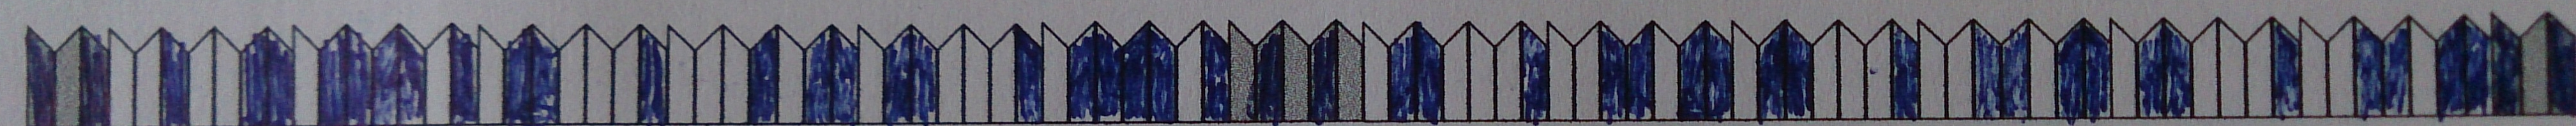
\includegraphics[height=1cm, width=16.5cm]{EANbearbeitet.jpg}
	\end{center}
\end{solution}

\problemnumber{5}
\begin{problem}
	Gegeben ist der nachfolgende Signalverlauf mit Pegel 1 (\emph{high}) und
	Pegel 2 (\emph{low}).
	\begin{center}
\begin{minipage}{0.1\textwidth}
	\large 
	Pegel 1 \\

	Pegel 2
\end{minipage}
\begin{minipage}{0.8\textwidth}
	\begin{center}
		\begin{tikzpicture}[x=1cm, y=1cm]
			\draw[step=1cm, black, thin, dotted, dot spacing=2pt] (-0.5,-0.5) grid (12.5, 1.5); % Hier Grid-Größe anpassen
			\draw[ultra thick] (-0.5, 0) -- (0, 0);
			\draw[ultra thick] (0, 0) -- (0, 1);
			\draw[ultra thick] (0, 1) -- (1, 1);
			\draw[ultra thick] (1, 1) -- (1, 0);
			\draw[ultra thick] (1, 0) -- (2, 0); % Hier Striche für die Lösung hinzufügen/verändern
			\draw[ultra thick] (2, 0) -- (2, 1);
			\draw[ultra thick] (2, 1) -- (3, 1);
			\draw[ultra thick] (3, 1) -- (3, 0);
			\draw[ultra thick] (3, 0) -- (4, 0);
			\draw[ultra thick] (4, 0) -- (5, 0);
			\draw[ultra thick] (5, 0) -- (6, 0);
			\draw[ultra thick] (6, 0) -- (6, 1);
			\draw[ultra thick] (6, 1) -- (7, 1);
			\draw[ultra thick] (7, 1) -- (8, 1);
			\draw[ultra thick] (8, 1) -- (9, 1);
			\draw[ultra thick] (9, 1) -- (9, 0);
			\draw[ultra thick] (9, 0) -- (10, 0);
			\draw[ultra thick] (10, 0) -- (10, 1);
			\draw[ultra thick] (10, 1) -- (11, 1);
			\draw[ultra thick] (11, 1) -- (12, 1);
			\draw[ultra thick] (12, 1) -- (12, 0);
			\draw[ultra thick] (12, 0) -- (12.5, 0);
		\end{tikzpicture}
	\end{center}
\end{minipage}
\end{center}
\begin{parts}
	\part 
	\label{5.a}
	Interpretieren Sie den Signalverlauf in NRZ-L-Codierung und geben Síe
	die decodierte 0/1-Folge an!
	\part 
	\label{5.b}
	Interpretieren Sie den Signalverlauf in NRZ-S-Codierung und geben Sie
	die decodierte 0/1-Folge an! Gehen Sie davon aus, dass die Folge bei Pegel
	\emph{low} mit Wert 0 startet.
	\part
	\label{5.c}
	Zeichnen Sie zum nachfolgend gegebenen Signalverlauf in NRZ-L-Codierung darunter
	den entsprechenden Signalverlauf in NRZ-M-Codierung! Gehen Sie davon aus, dass NRZ-M
	mit Pegel \emph{high} startet.
\end{parts}

\end{problem}
\begin{solution}
	\ref{5.a}
	\[\text{Decodierter Signalverlauf: }01010001110110\]

	\ref{5.b}
	\[\text{Decodierter Signalverlauf: }00000110110010\]

	\ref{5.c}
	\[\text{Decodierter Signalverlauf: }01001110000101\]
	
	\begin{center}
	\begin{minipage}{0.1\textwidth}
		\large 
		NRZ-M
	\end{minipage}
	\begin{minipage}{0.8\textwidth}
		\begin{center}
			\begin{tikzpicture}[x=1cm, y=1cm]
				\draw[step=1cm, black, thin, dotted, dot spacing=2pt] (-0.5,-0.5) grid (11.5, 1.5); % Hier Grid-Größe anpassen
				\draw[ultra thick] (-0.5, 1) -- (0, 1);
				\draw[ultra thick] (0, 1) -- (0, 0);
				\draw[ultra thick] (0, 0) -- (1, 0);
				\draw[ultra thick] (1, 0) -- (2, 0);
				\draw[ultra thick] (2, 0) -- (3, 0); % Hier Striche für die Lösung hinzufügen/verändern
				\draw[ultra thick] (3, 0) -- (3, 1);
				\draw[ultra thick] (3, 1) -- (4, 1);
				\draw[ultra thick] (4, 1) -- (4, 0);
				\draw[ultra thick] (4, 0) -- (5, 0);
				\draw[ultra thick] (5, 0) -- (5, 1);
				\draw[ultra thick] (5, 1) -- (6, 1);
				\draw[ultra thick] (6, 1) -- (7, 1);
				\draw[ultra thick] (7, 1) -- (8, 1);
				\draw[ultra thick] (8, 1) -- (9, 1);
				\draw[ultra thick] (9, 1) -- (9, 0);
				\draw[ultra thick] (9, 0) -- (10, 0);
				\draw[ultra thick] (10, 0) -- (11, 0);
				\draw[ultra thick] (11, 0) -- (11, 1);
				\draw[ultra thick] (11, 1) -- (11.5, 1);
			\end{tikzpicture}
		\end{center}
	\end{minipage}
	\end{center}
\end{solution}

\newpage

\problemnumber{7}
\begin{problem}
	Gegeben ist ein Code mit fünf Codewörtern: 0011001, 0010101, 1101011, 0001111 und 1010100.
	\begin{parts}
		\part
		\label{7.a}
		Berechnen Sie die Hamming-Distanz zwischen den einzelnen Codewörtern und vervollständigen
		Sie die nachfolgende Distanz-Matrix!
		\begin{center}
		\begin{tabular}{|c|c|c|c|c|c|}
			\hline
			        & 0011001 & 0010101 & 1101011 & 0001111 & 1010100 \\ \hline
			0011001 & 0       & 2       & 4       & 3       & 4       \\ \hline
			0010101 & 2       & 0       & 6       & 3       & 2       \\ \hline
			1101011 & 4       & 6       & 0       & 3       & 6       \\ \hline
			0001111 & 3       & 3       & 3       & 0       & 5       \\ \hline
			1010100 & 4       & 2       & 6       & 5       & 0       \\ \hline
		\end{tabular}
		\end{center}
		\part 
		\label{7.b}
		Geben Sie den Hamming-Abstand $D$ des Codes an!
		\part 
		\label{7.c}
		Wie viele Bits braucht man mindestens, um einen Code für sechs Codewörter zu entwerfen,
		der einen Hamming-Abstand von $D=2$ aufweist?
	\end{parts}
\end{problem}
\begin{solution}
	\ref{7.a}
	Siehe Angabe! \\

	\ref{7.b}
	\centering Hamming Abstand $D = 2$
\end{solution}

\begin{problem}
	Es soll ein Hamming-Code für 4 Datenbits konstruiert werden.
	\begin{parts}
		\part 
		\label{8.a}
		Wie viele Prüfbits werden benötigt? Wie hoch ist die Anzahl der resultierenden Codebits?

		\part 
		\label{8.b}
		Wie lauten die Gleichungen für die nötigen Prüfbits dieses Codes?

		\part 
		\label{8.c}
		Listen Sie alle gültigen Codewörter dieses Codes in einer Tabelle auf!

		\part 
		\label{8.d}
		Überprüfen Sie anhand von zwei Beispielen, ob es sich um einen linearen Code handeln könnte!

		\part 
		\label{8.e}
		Decodieren und ggf. korrigieren Sie das empfangene Codewort 1101110 unter der Annahme, dass
		maximal ein Bit gestört wurde!

		\part 
		\label{8.f}
		Decodieren und ggf. korrigieren Sie das empfangene Codewort 1110110 unter der Annahme, dass
		maximal ein Bit gestört wurde!
	\end{parts}
\end{problem}

\begin{solution}
	\ref{8.a}
	Es werden 3 Prüfbits benötigt und die Anzahl der resultierenden Codebits beträgt 7. \\

	\ref{8.b}
	\[p_1 = c_1 = (c_3+c_5+c_7) \text{ mod } 2 = c_3 \otimes c_5 \otimes c_7\]
	\[p_2 = c_2 = (c_3+c_6+c_7) \text{ mod } 2 = c_3 \otimes c_6 \otimes c_7\]
	\[p_3 = c_4 = (c_5+c_6+c_7) \text{ mod } 2 = c_5 \otimes c_6 \otimes c_7\]
\newpage
	\ref{8.c}
	\begin{center}
		\begin{tabular}{|c|c|c|c|c|c|c|}
			\hline
			$c_1$ & $c_2$ & $c_3$ & $c_4$ & $c_5$ & $c_6$ & $c_7$ \\ \hline
			0     & 0     & 0     & 0     & 0     & 0     & 0     \\ \hline
			1     & 1     & 0     & 1     & 0     & 0     & 0     \\ \hline
			1     & 0     & 1     & 0     & 1     & 0     & 0     \\ \hline
			0     & 1     & 1     & 1     & 1     & 0     & 0     \\ \hline
			0     & 1     & 1     & 0     & 0     & 1     & 0     \\ \hline
			1     & 0     & 1     & 1     & 0     & 1     & 0     \\ \hline
			1     & 1     & 0     & 0     & 1     & 1     & 0     \\ \hline
			0     & 0     & 0     & 1     & 1     & 1     & 0     \\ \hline
			1     & 1     & 1     & 0     & 0     & 0     & 1     \\ \hline
			0     & 0     & 1     & 1     & 0     & 0     & 1     \\ \hline
			0     & 1     & 0     & 0     & 1     & 0     & 1     \\ \hline
			1     & 0     & 0     & 1     & 1     & 0     & 1     \\ \hline
			1     & 0     & 0     & 0     & 0     & 1     & 1     \\ \hline
			0     & 1     & 0     & 1     & 0     & 1     & 1     \\ \hline
			0     & 0     & 1     & 0     & 1     & 1     & 1     \\ \hline
			1     & 1     & 1     & 1     & 1     & 1     & 1     \\ \hline
		\end{tabular}
	\end{center}

	\ref{8.d}
	\[ (0110010 + 1011010) \text{ mod } 2 = 0000000 \]
	\[ (0010111 + 0100101) = 00111100 \]

	\ref{8.e}
	\[ p_1 = c_1 = 0 \otimes 1 \otimes 0 = 1 = 1 \quad \checkmark \]
	\[ p_2 = c_2 = 0 \otimes 1 \otimes 0 = 1 = 1 \quad \checkmark \]
	\[ p_3 = c_4 = 1 \otimes 1 \otimes 0 = 0 \neq 1 \quad \text{\lightning} \]
	\begin{center}
		$c_4$ gestört! Richtig: 1100110
	\end{center}

	\ref{8.f}
	\[ p_1 = c_1 = 1 \otimes 1 \otimes 0 = 0 \neq 1 \quad \text{\lightning} \]
	\[ p_2 = c_2 = 1 \otimes 1 \otimes 0 = 0 \neq 1 \quad \text{\lightning} \]
	\[ p_3 = c_4 = 1 \otimes 1 \otimes 0 = 0 = 0 \quad \checkmark \]
	\begin{center}
		$c_3$ gestört, weil $(1+2) = 3$! Richtig: 1100110
	\end{center}
\end{solution}

\end{document}